\documentclass[pdf]{beamer}
\usepackage[latin1]{inputenc}
\usepackage{multirow}
\usetheme{AnnArbor} %Warsaw
\usecolortheme{beaver}

%\documentclass[pdf]{beamer}
%\usepackage[latin1]{inputenc}
%\usepackage{multirow}
%\usetheme{Warsaw} %Warsaw
%\usecolortheme{beetle}

\begin{document}

\title[BCB 504-Microarrays]{Custom microarray analysis in R}
\author[Matt Settles]{Matt Settles}
\institute{University of Idaho\\Bioinformatics and Computational Biology Program}
\date{\today}


%% Title page
\begin{frame}[plain]
  \titlepage
\end{frame}


%% Outline
\begin{frame}[plain] 
  \frametitle{Outline}
  \tableofcontents
\end{frame}

\section{Analysis Setup}
\begin{frame}
  \begin{itemize}
    \item \structure{Experiment\_Directory}
    \begin{itemize}
      \item \structure{Raw\_Data}
      \item \structure{Design\_Files}
      \item \structure{Figures}
      \item \structure{Tables}
      \item \structure{Data}
      \item Analysis.R
      \item Venn.R
      \item functions.R
      \item targets.txt
    \end{itemize}
  \end{itemize}
\end{frame}

\begin{frame}
  \frametitle{targets.txt - an annotated data frame}
  An annotated data frame allows you to manage the samples for the experiment and includes at minimum sample names with associated raw data files. The framework however is flexible and allows for more information about samples to be included.\\


 \alert{See targets.txt file in example data} 
\end{frame}
  
\section{Raw Data}
\begin{frame} 
  \frametitle{Components of Raw Data}
  \begin{itemize}
    \item Quantified intensities for each microarray probe (spot), usually identified by X,Y coordinate
    \begin{description}
      \item[Affymetrix] binary CEL files
      \item[Nimblegen] plain text pair or xys files
      \item[Agilent] plain text gpr files 
    \end{description}
    \item Microarray description file, associates probes to probesets and genes
    \begin{description}
      \item[Affymetrix] CEL description files or CDF files (Bioconductor provides)
      \item[Nimblegen] Nimblegen description files or NDF files (must create your own packages)
      \item[Agilent] GAL files (can be used in Limma)
    \end{description}
  \end{itemize}
\end{frame}

%
\section{Quality Assurance}
\begin{frame}
  \frametitle{Quality Assurance}
  \begin{enumerate}
    \item Visual check of chip images or pseudo-images.
    \item Consistency across microarrays.
    \item Observed patterns meet expectations.
  \end{enumerate}
\end{frame}

\subsection{Chip Images}
\begin{frame}
  \frametitle{Pseudo-chip images}
  \begin{columns}[t] % contents are top vertically aligned
    \begin{column}[T]{5cm} % each column can also be its own environment
      \begin{itemize}
        \item Pseudo-chip images are created from the data themselves and not from the original scanned images
        \item Can be created from the raw intensities, log intensities, model fitting residuals and other
        \item Looking for large anomalies
      \end{itemize}
     \end{column}
     \begin{column}[T]{5cm} % alternative top-align that's better for graphics
        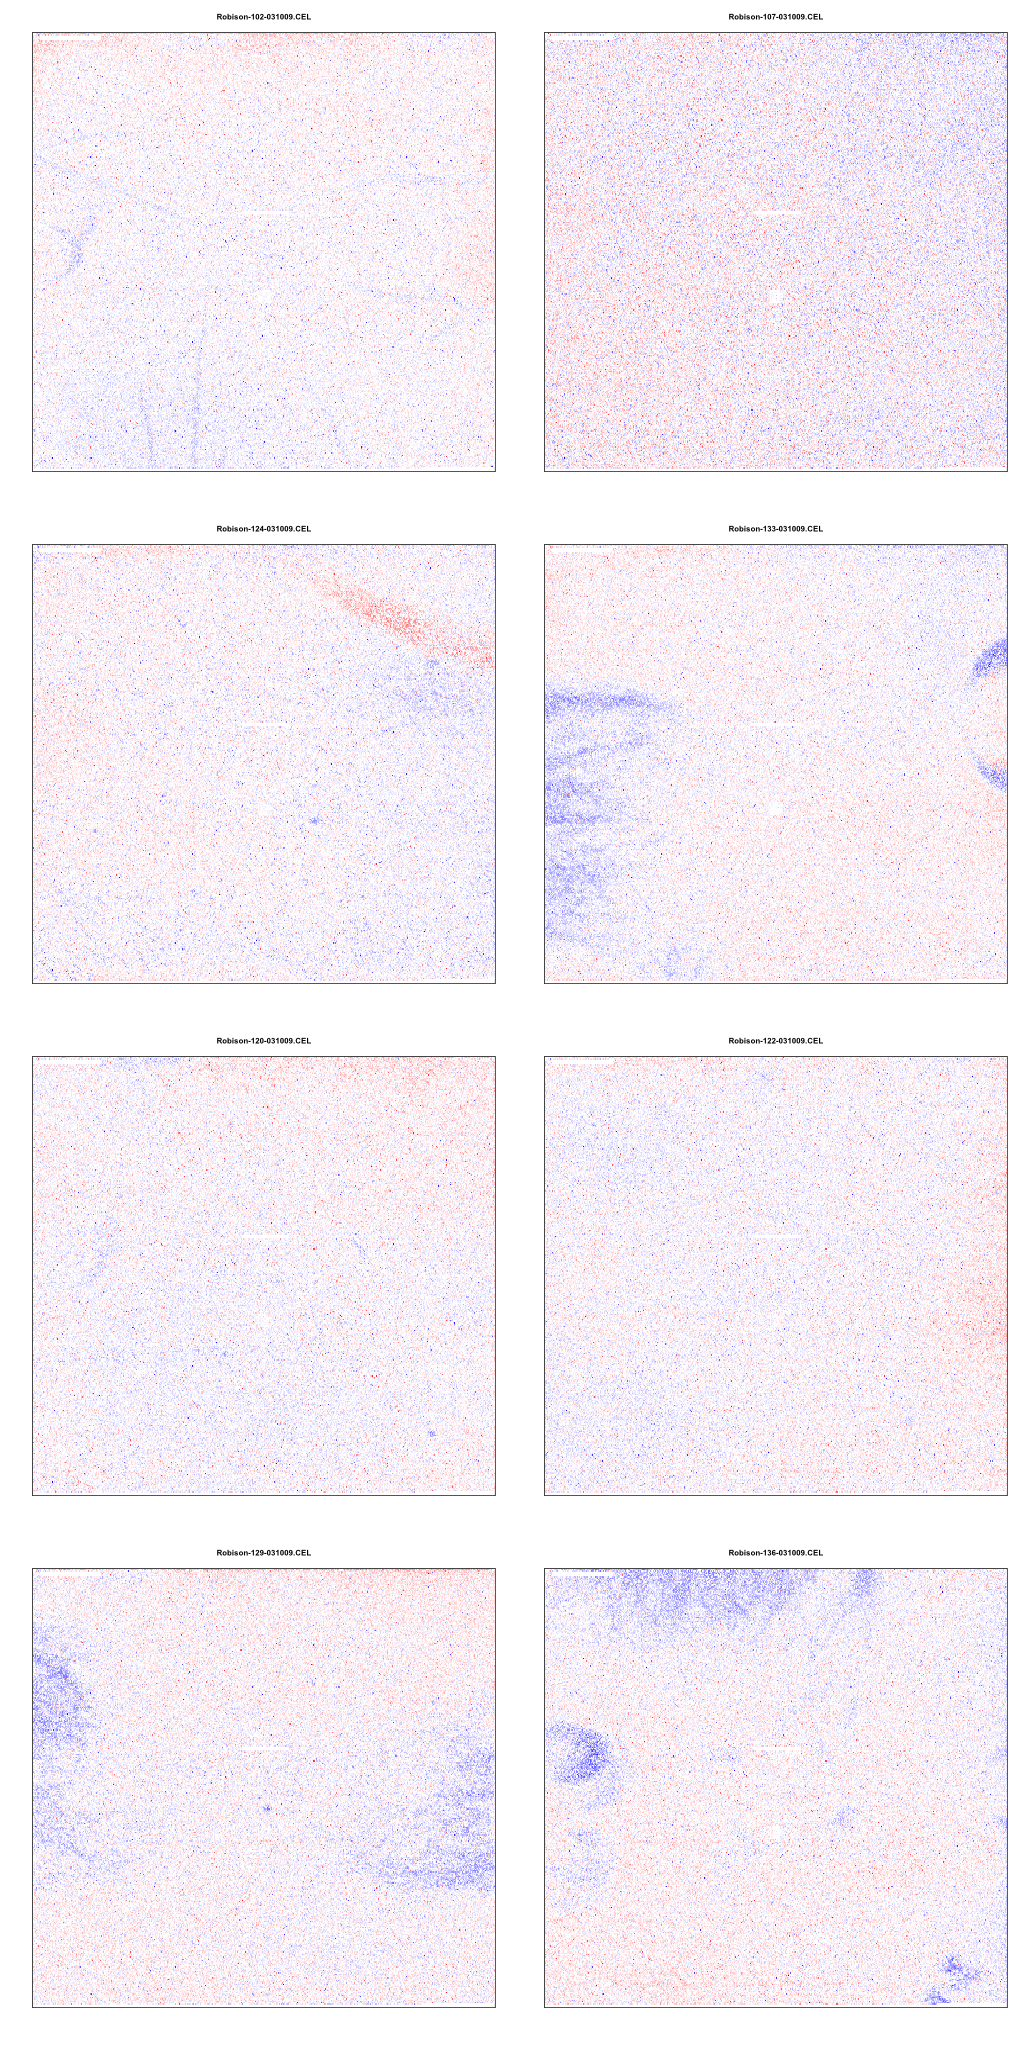
\includegraphics[scale=0.09]{figures/resid0.png} 
     \end{column}
  \end{columns}
\end{frame}

\subsection{Consistency}
\begin{frame}
  \frametitle{Consistency across microarrays}
  \begin{center}
  \centering 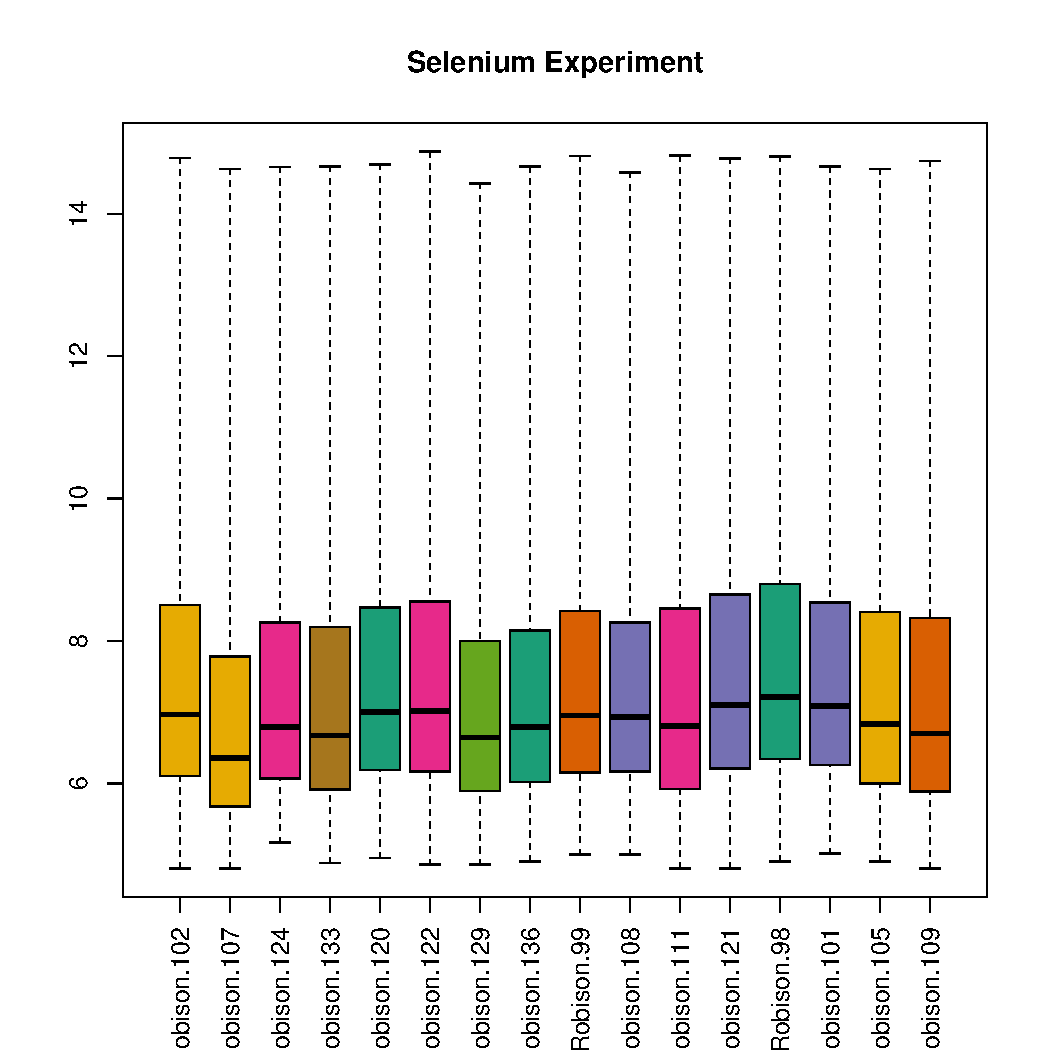
\includegraphics[scale=0.40]{figures/affybxp.pdf}
  \end{center}
\end{frame}

\begin{frame}
  \begin{center}
  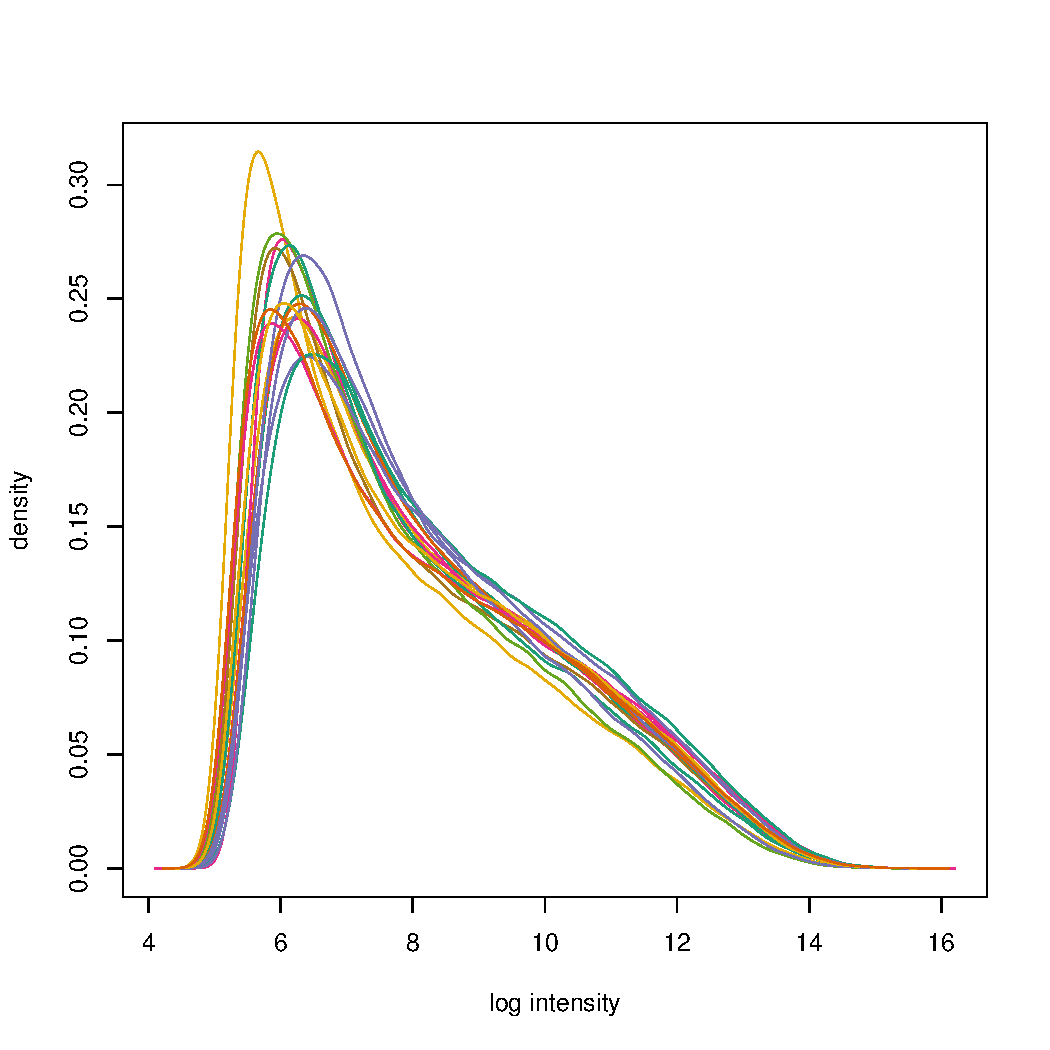
\includegraphics[scale=0.45]{figures/affyhist.pdf}  
  \end{center}
\end{frame}

\subsection{Expectations} 

\begin{frame}
  \frametitle{Expectations}  
  \begin{center}
  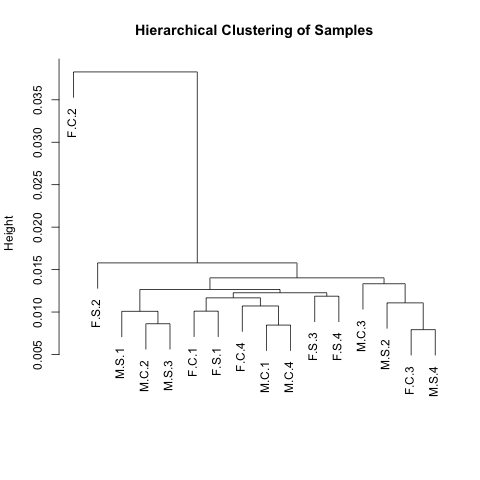
\includegraphics[scale=0.45]{figures/Figure3.png} 
  \end{center}
\end{frame}


\section{Preprocessing}
\begin{frame}
  \frametitle{Preprocessing}
  The goals of preprocessing Affymetrix microarray data are three fold:
  \begin{enumerate}
    \item To remove variation due to technical sources, while preserving variation from biological sources. 
    \item To normalize a set of microarrays in order to make them comparable.
    \item To produce summarized expression values for each probe set.
  \end{enumerate} 
\end{frame}

\begin{frame}
  \begin{description}
    \item[Background correction] Local Effects. Deviations from actual expression levels are introduced by many sources including scanner artifacts, non-specific binding (hybridization), RNA quality, reagents, etc.. All of which can be considered as background noise.
    \item[Probe level normalization] Array Effects. The role of normalization is to compensate for the technical effects, while preserving the effects due to the biology.
    \item[PM Correction] PM correction routines are designed to account for non-specific binding by use of the MM probes.
    \item[Probe set summarization] Probe set summarization produces a single value for a probe set that is the estimated expression level for the probe set (i.e. gene).
    \item[Probe set normalization] Same purpose as Probe level normalization but on the probe sets.
  \end{description}
\end{frame}

\subsection{Algorithms}
\begin{frame}
  \begin{tiny}
  \begin{center}
  \begin{table}
  \caption{Breakdown of the preprocessing steps for the MAS5, Plier, RMA, GCRMA, and dChip preprocessing pipelines.}
  \begin{tabular}{|l|c|c|c|c|c|}
  \hline
  & \textbf{MAS5} & \textbf{Plier} & \textbf{RMA} & \textbf{GCRMA} & \textbf{dChip} \\ \hline
  Background & weighted   & \multirow{2}{*}{none} & RMA  & GCRMA & \multirow{2}{*}{none} \\
  Correction &  average  &  & (global model) & (model based) &  \\ \hline
  Probe Level &  \multirow{2}{*}{none}   & quantile  &  quantile  &  quantile  & invariant  \\
  Normalization  & &  normalization &   normalization &   normalization &  set\\ \hline
    \multirow{2}{*}{PM Correction} & ideal & \multirow{2}{*}{none} & \multirow{2}{*}{none} & \multirow{2}{*}{none} & subtract MM \\ 
    &  mismatch    & & & & none \\ \hline
  Probe set & Tukey & \multirow{2}{*}{Plier} & median  & median  & \multirow{2}{*}{MBEI}\\  
  Summarization &  biweight   &  &  polish &  polish &  \\ \hline
  Probe set & mean & \multirow{2}{*}{none} & \multirow{2}{*}{none} & \multirow{2}{*}{none} & \multirow{2}{*}{none}\\ 
  Normalization & scaled &  &  &  & \\ \hline
  \end{tabular}
  \end{table}
  \end{center}
  \end{tiny}
\end{frame}
   
\subsection{QA preprocessing}
\begin{frame}
\begin{center}
  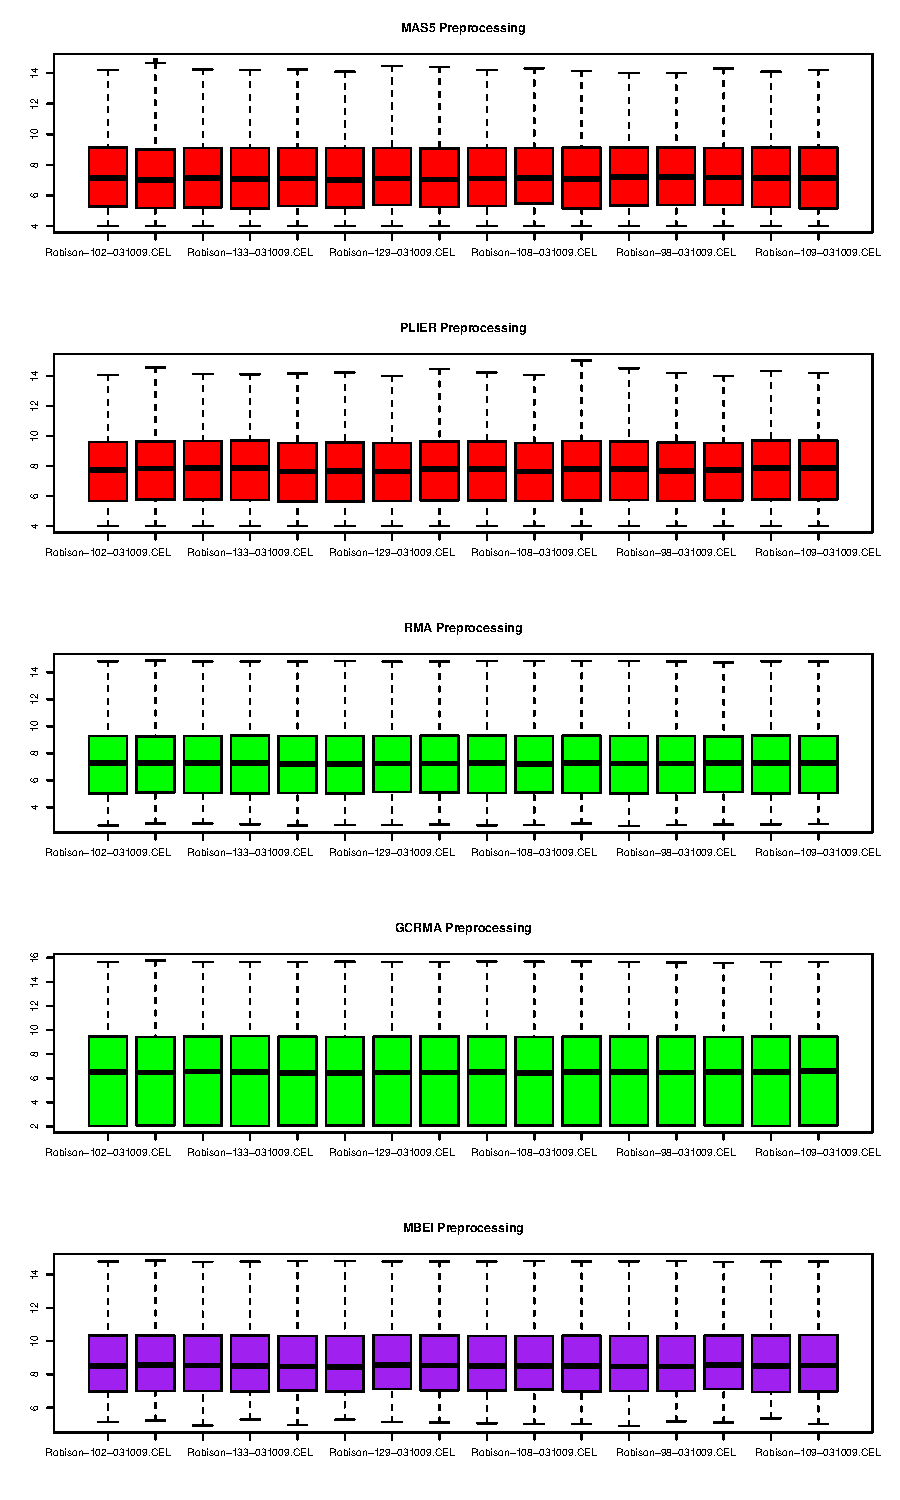
\includegraphics[scale=0.4]{figures/normboxplots.pdf} 
\end{center}
\end{frame}

\begin{frame}
\begin{center}
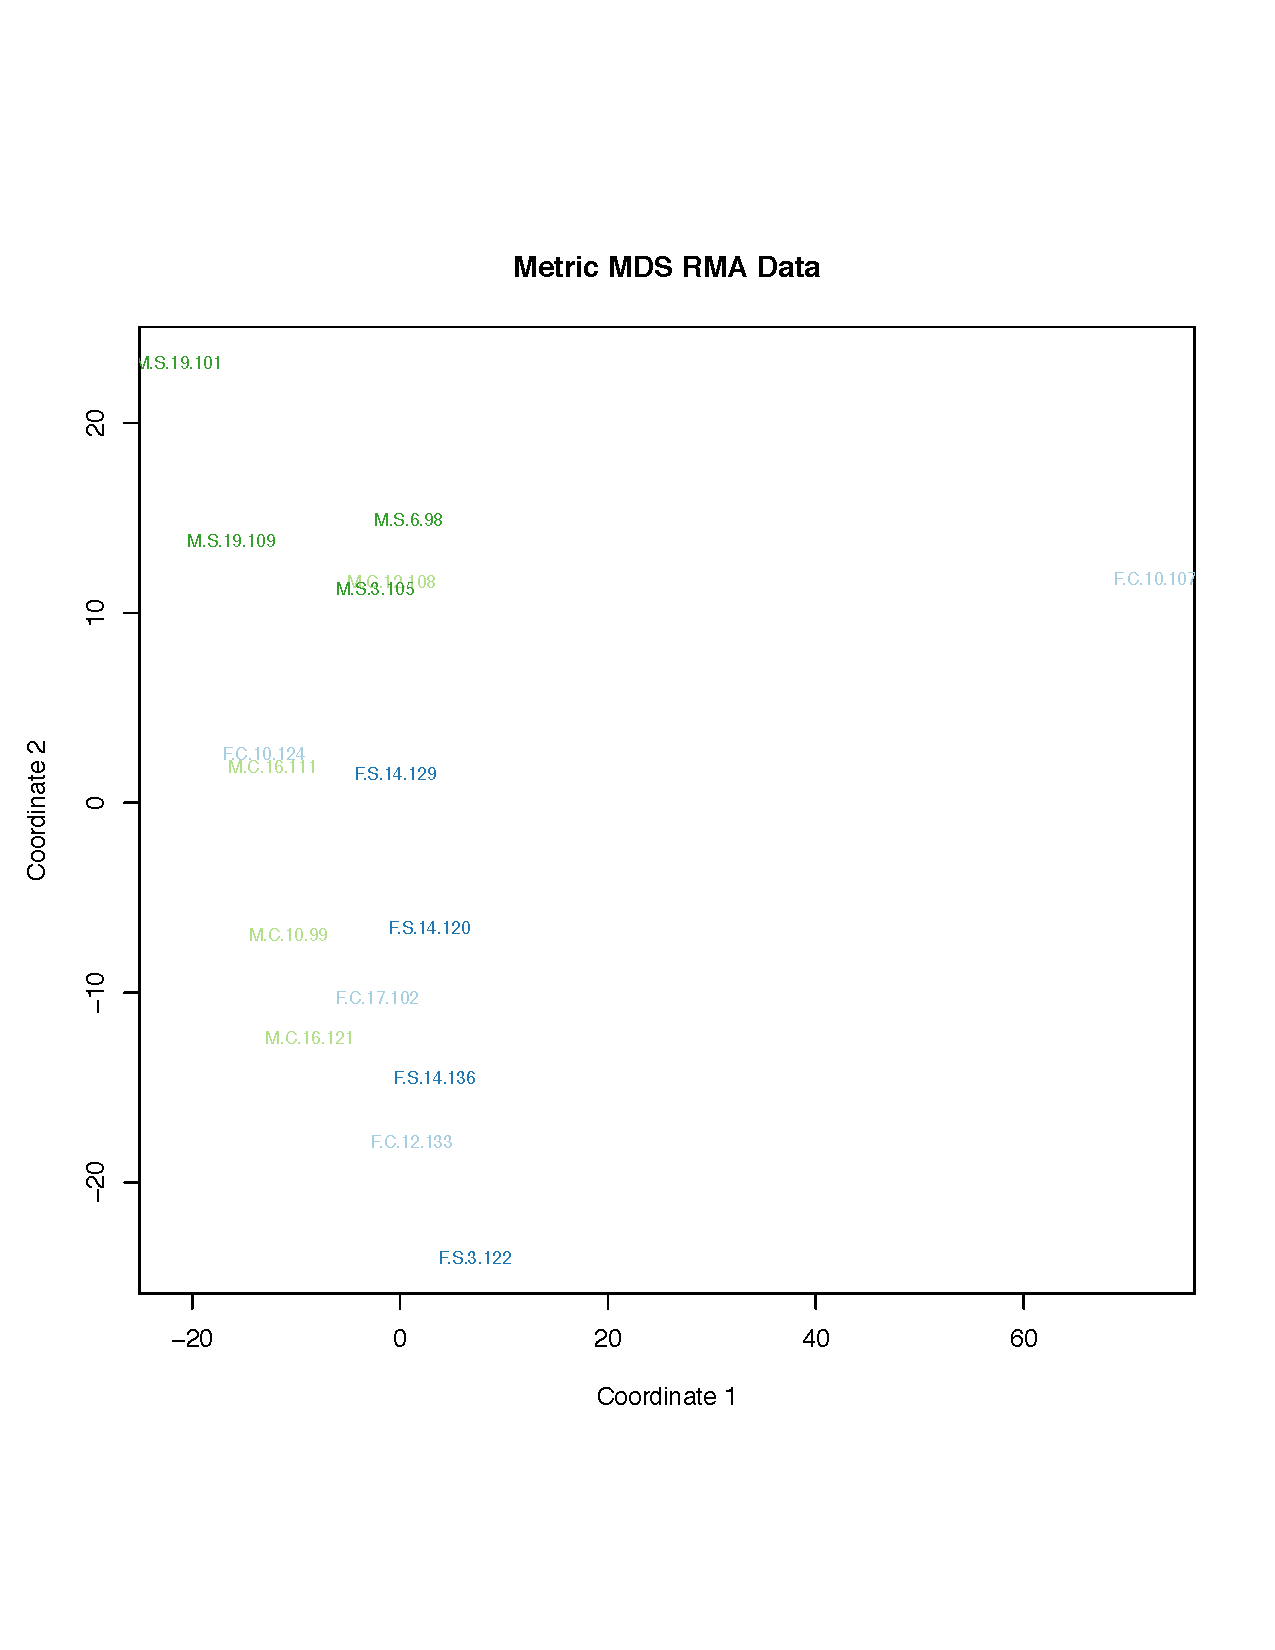
\includegraphics[scale=0.3]{figures/normMDS.pdf} 
\end{center}
\end{frame}

\section{Robust Multichip Averaging (RMA)}

\begin{frame}
  \frametitle{RMA}
  \begin{itemize}
  \item \href{http://biostatistics.oxfordjournals.org/content/4/2/249.abstract}{Irizarry et al. (2003) Biostatistics 4(2):249-264.}
  \item \href{http://nar.oxfordjournals.org/content/31/4/e15.abstract}{Irizarry et al. (2003) Nucleic Acids Research 31(4):e15.}
  \item \href{http://bioinformatics.oxfordjournals.org/content/19/2/185.abstract}{Bolstad et al. (2003) Bioinformatics 19(2):185-193.}
  \end{itemize}
\end{frame}

\begin{frame}
  \frametitle{RMA-Convolutation Background Correction}
\begin{center}
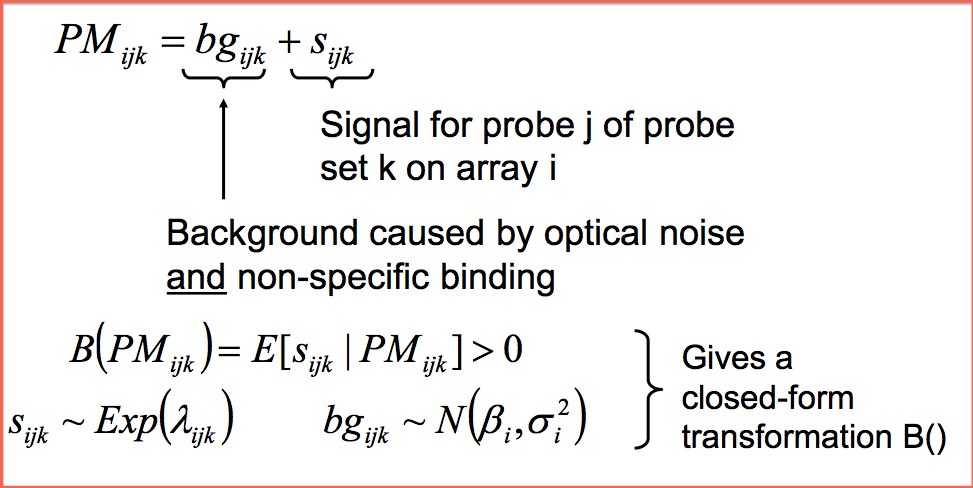
\includegraphics[scale=0.3]{figures/RMA-background.png} 
\end{center}
\end{frame}

\begin{frame}
  \frametitle{RMA-Quantile Normalization}
A technique for making two or more distributions identical in statistical properties.
\begin{itemize}
\item Each vector to be normalized must be the same length
\item Sort the vectors from smallest to greatest.
\item Compute the means at each sorted column, this is the new distribution.
\item Unsort the original vectors using the new computed distribution.
\end{itemize}
Note: Assumes, they should have the same underlying distributions.
\end{frame}

\begin{frame}
  \frametitle{RMA-Median Polosh}
Robust method suggested by Tukey for estimating the mean, row and column parameters of the model
\begin{center}
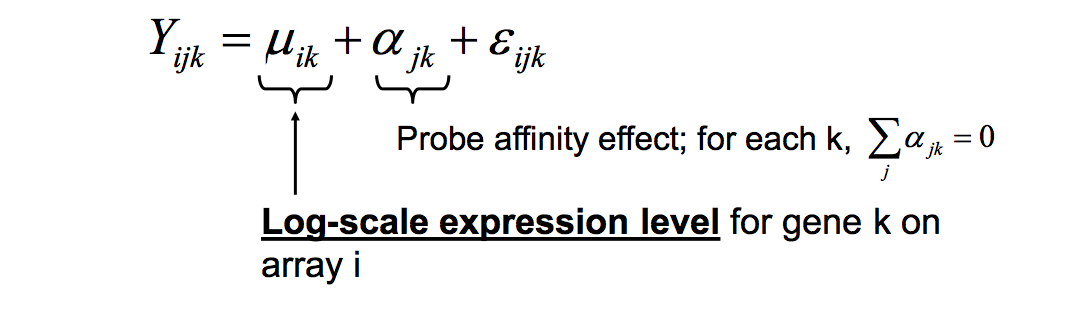
\includegraphics[scale=0.3]{figures/RMA-medianpolish.png} 
\end{center}
\end{frame}

\section{Data filtering}

\begin{frame}
  \frametitle{Gene filtering}
  Purpose is to remove probe sets (aka genes) that are likely to be of no use (uninteresting) when modelling the data.
  \begin{description}
  \item[non-specific] Choose genes to remove (or keep) without using any phenotypic variables in the filtering process. Result can then be used with any downstream process without bias.
  \item[specific] Use of experimental variables to choose which genes should be kept/removed. Results can be used in a descriptive nature, should not be used for statistical testing.
 \end{description}
\end{frame}

\begin{frame}[allowframebreaks,fragile]
  \frametitle{Non-specific filters}
  \begin{description}
  \item [Annotation Based Filtering] Can reduce be a predetermined set of genes (aka entrez ids), by Gene Ontology group, filter based on available annotation data. 
  \item [Duplicate Probe Removal] Probes determined by annotation to be pointing to the same gene are compared, and only the probe with the highest variance value will be retained.
  \item [Variance Based Filtering] Perform numerical cutoff-based filtering (aka IQR). The intention is to remove uninformative probe sets, representing genes that were not expressed at all or no change is occurring. Observations  have shown that unexpressed genes are detected most reliably through their low variability across samples. IQR is robust to outliers, a default cutoff value of 0.5 is motivated by the rule of thumb that in many tissues only 40\% of genes are expressed.
  \end{description}
\end{frame}
%

\section{Differential Expression}
\begin{frame}[allowframebreaks,fragile]
  \frametitle{Differential Expression Analysis}
  \begin{description}
  \item [LIMMA] Linear Models for Microarray Data approach. Limma applies a linear model to the data and uses model contrasts to extract specific comparisons of interest. It then uses multiple testing correction based techniques (FDR, FWER, etc.) for MT corrected p-values. Can also choose a fold change parameter, to ensure that called genes change at least a pre-specified amount. 
  \end{description}
\end{frame}

\subsection{Variance Stabilization}


\begin{frame}
  \frametitle{Variance Stabilization}
  \begin{itemize}
  \item When doing statistical test, we estimate the variance for each gene individually. This is fine, \textit{if} we have enough replicates, but with few replicages (say 3-5 per group), these variances are highly variable.
  \item In a moderated statistic, the estimated gene-specific variance $s^2_g$ is replaced by a weighted average of $s^2_g$ and $s^2_0$, which is a global variance estimator obtained from pooling all genes.
  \item This produces an interpolation between the t-test and a fold-change criterion.
  \end{itemize}
LIMMA performs an empirical Bayes estimate for $s^2_0$.
\end{frame}

\subsection{Multiple Testing Correction}
\begin{frame}
  \frametitle{FWER vs FDR}
  \textbf{Aim:} For a given type I error rate $\alpha$, use a procedure to select a set of "significant" genes that guarantees a type I error rate less than or equal to $\alpha$.   
  \begin{description}
  \item[FWER] Familywise Error Rate - is the probability of making one or more false discoveries, or type I errors among all the hypotheses when performing multiple hypotheses tests. Stringent test such as Bonferonni.
  \item[FDR] False Discovery Rate - In a list of statistically significant findings, FDR procedures are designed to control the expected proportion of incorrectly rejected null hypotheses ("false discoveries"). Less stringent test such as BH and q-value.
  \end{description}
\end{frame}

\begin{frame}
  \frametitle{Multiple Testing Correction}
  Many methods available in the bioconductor packages \textit{multtest} and \textit{qvalue}.
  \begin{description}
  \item[Bonferonni] Basically multiple raw p-value by the number of tests. \textbf{Unrealistic} given the number of genes tested.
  \item [Benjimini and Hochberg (BH)] Controls the false discovery rate. Works for independent test statistics and for some types of dependence. Tends to be conservative if many genes are differentially expressed.  
  \item [q-value] the q-value of a gene is defined as the minimal estimated FDR at which it appears significant.
  \end{description}
\end{frame}

\section{Public Repositories}
\begin{frame}
  \frametitle{Public Repositories for Microarrays Data}
  \begin{description}
    \item[GEO] \href{http://www.ncbi.nlm.nih.gov/geo/}{http://www.ncbi.nlm.nih.gov/geo/}
	\newline
    \item[ArrayExpress] \href{http://www.ebi.ac.uk/arrayexpress/}{http://www.ebi.ac.uk/arrayexpress/}
  \end{description}  
\end{frame}

\end{document}

